\chapter{Results}

% D.
% intro text, please

In this chapter, we will present our experimental results. Our first experiment shows that the prediction accuracy of our system is better than existing state-of-the-art models. In the second experiment, we aim to find the optimal number of hidden dimensions.

\section{Experiment Results}

\begin{table}[htbp!]
\centering
 \begin{tabular}{||c c c c c c c||} 
 \hline
  & hitrate@1 & hitrate@5 & hitrate@10 & NDCG@5 & NDCG@10 & MAP\\ [0.5ex] 
 \hline\hline
 BERT4Rec & \underline{0.3458} & \underline{0.6630} & 0.7667 & \underline{0.5156} & \underline{0.5493} & \underline{0.4905} \\ 
 %\hline
 Caser & 0.3276 & 0.6591 & \underline{0.7761} & 0.5038 & 0.5418 & 0.4780 \\
 %\hline
 FPMC & 0.2599 & 0.5812 & 0.7230 & 0.4287 & 0.4749 & 0.4103 \\
 \hline
 Hybrid & \textbf{0.3645} & \textbf{0.6855} & \textbf{0.7847} & \textbf{0.5377} & \textbf{0.5698} & \textbf{0.5197} \\ 
 %\hline 
 Accuracy Gain & 5.26\% & 3.39\% & 1.10\% & 4.28\% & 3.73\% & 5.95\% \\
 \hline
\end{tabular}
\caption{Hybrid accuracy metrics, MovieLens 1M}
\label{tab:accuracy_hybrid_movielens}
\end{table}

\begin{figure}[htbp!]
\centering
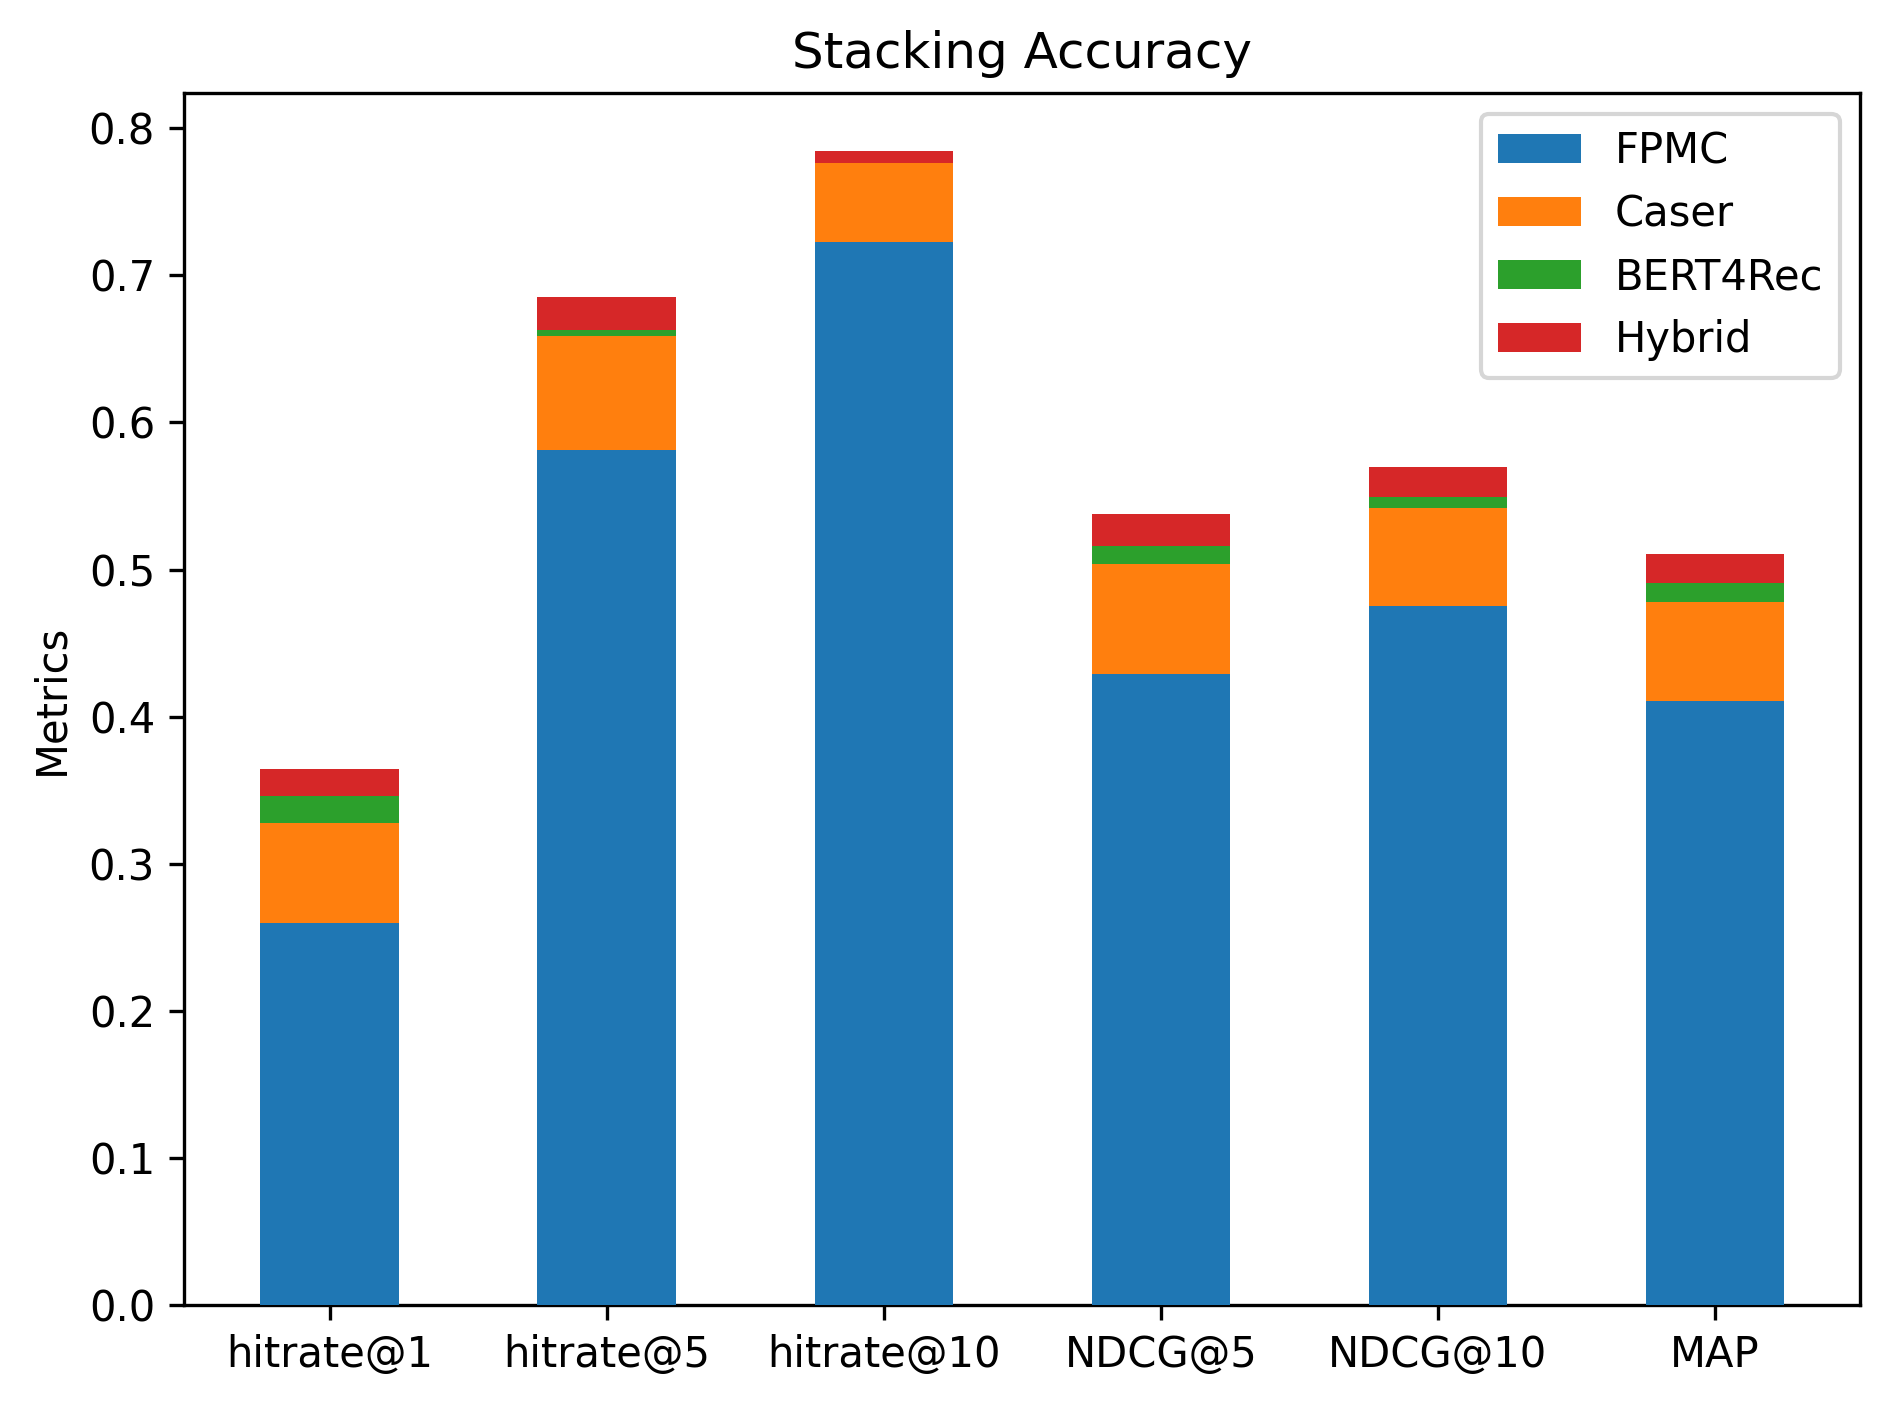
\includegraphics[width=0.8\textwidth]{images/plots/stacking_accuracy_movielens.png}
\caption{Illustration showing accuracy gain of out hybrid model compared to state of the art models for the dataset MovieLens 1M}
\label{fig:accuracy_hybrid_movielens}
\end{figure}

\begin{table}[htbp!]
\centering
 \begin{tabular}{||c c c c c c c||} 
 \hline
  & hitrate@1 & hitrate@5 & hitrate@10 & NDCG@5 & NDCG@10 & MAP\\ [0.5ex] 
 \hline\hline
 BERT4Rec & \underline{0.1658} & \underline{0.3516} & \underline{0.4593} & \underline{0.262} & \underline{0.2968} & \underline{0.2646} \\ 
 %\hline
 Caser & 0.1144 & 0.2798 & 0.3996 & 0.2083 & 0.2270 & 0.1991 \\
 %\hline
 FPMC & 0.1070 & 0.2693 & 0.3715 & 0.1906 & 0.2235 &  0.1977 \\
 \hline
 Hybrid & \textbf{0.1755} & \textbf{0.3631} & \textbf{0.4663} & \textbf{0.2743} & \textbf{0.3034} & \textbf{0.276} \\ 
 %\hline 
 Accuracy Gain & 5.85\% & 3.27\% & 1.52\% & 4.69\% & 2.22\% & 4.31\% \\
 \hline
\end{tabular}
\caption{Hybrid accuracy metrics, Amazon Beauty}
\label{tab:accuracy_hybrid_beauty}
\end{table}

\begin{figure}[htbp!]
\centering
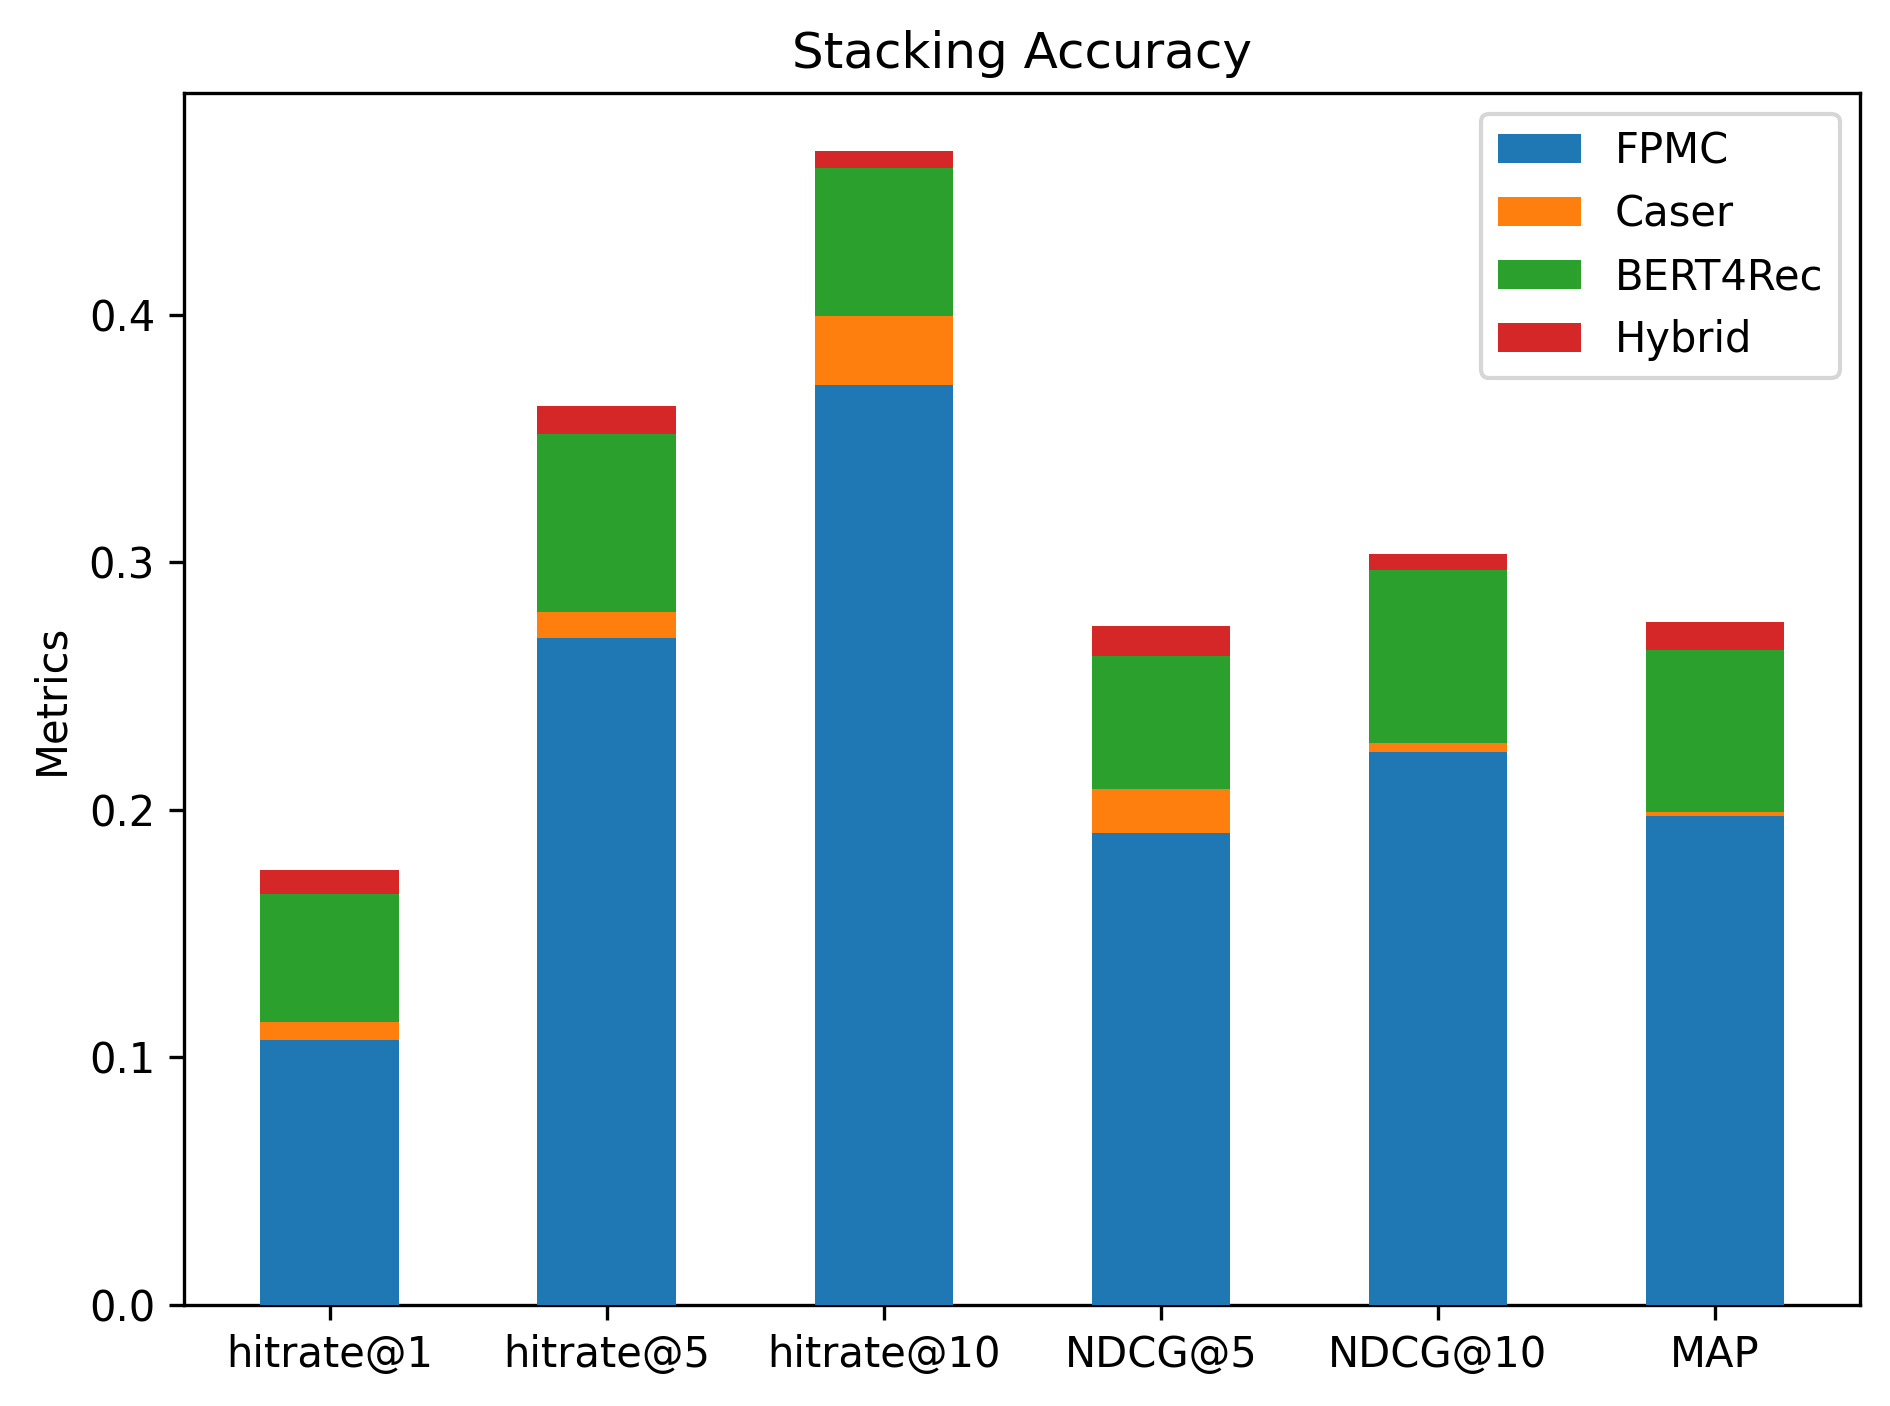
\includegraphics[width=0.8\textwidth]{images/plots/stacking_accuracy_beauty.png}
\caption{Illustration showing accuracy gain of out hybrid model compared to state of the art models for the dataset Amazon Beauty}
\label{fig:accuracy_hybrid_beauty}
\end{figure}

% 1. Say we want to investigate sth. and why it will bring us useful insights.
In our first experiment, we want to investigate how accurate the predictions of our hybrid system are. In the literature, authors often present the accuracy of their recommender systems to demonstrate the performance\cite{sun2019bert4rec,rendlefactorizing}. We also want to investigate if our system is more accurate than existing state-of-the-art models. Finally, since we have built a hybrid system, we want to compare our results to a non-hybrid version to ensure that the hybridization was useful.

% 2. Say how we investigate that thing, i.e., experimental setup.
To demonstrate the advantage of our hybrid system, we compare the results to several state-of-the-art recommender models. For fair evaluation, we follow the same evaluation procedure for every model. 
We do so using our online setup and explore the performance for various dynamics of the subcomponents, from small batches with close to no re-training per batch to large batches with heavy re-training. We also let the degree of control vary from highly automated (extensive exploration of the parameter space by the machine) to highly manual (conservative setting of the parameters by the humans). And finally, using more efficient meta-learning methods for the meta optimization. We do this to increase the accuracy of predictions while at the same time reducing the configuration overhead. For evaluation, we follow the procedure presented in Section~\ref{sec:test_procedure} and let our system predict the last item in the sequence of every user. We use the evaluation metrics presented in Section~\ref{sec:metrics}. Both evaluation procedure and evaluation metrics follow common standards used for evaluation in popular papers of state-of-the-art models. 

% 3. Say our results are presented in Material XYZ (plot/table)
We present our results for both our datasets in the Tables~\ref{tab:accuracy_hybrid_movielens},~\ref{tab:accuracy_hybrid_beauty} and a visualization in the Figures~\ref{fig:accuracy_hybrid_movielens},~\ref{fig:accuracy_hybrid_beauty}. In the tables, we can see the evaluation metrics and how each baseline model scores in our experiment compared to the score of our hybrid system. Underlined for every metric is the score of the baseline model that performs the best. 

% 4. describe the results. Just tell us what are the most striking patterns
If we compare the scores of our hybrid system to the baseline scores, we can see that our system can significantly outperform the other models. For the MovieLens 1M dataset, we can see a 5.26\% improvement of the hitrate@1 and a 5.95\% improvement of the MAP. We note an increase of 5.85\% of the hitrate@1 and a 4.31\% increase of the MAP for the Amazon Beauty dataset. 

% 5. discuss the results. Try to explain what we saw
Overall the results confirm that our hybrid system is significantly more accurate than the individual models. The improvement is large enough to warrant the extra effort in developing the system. We believe that we could further improve the system by adding more models in the future.


\section{Optimizing Hidden Dimensions}

\begin{figure}[htbp!]
\centering
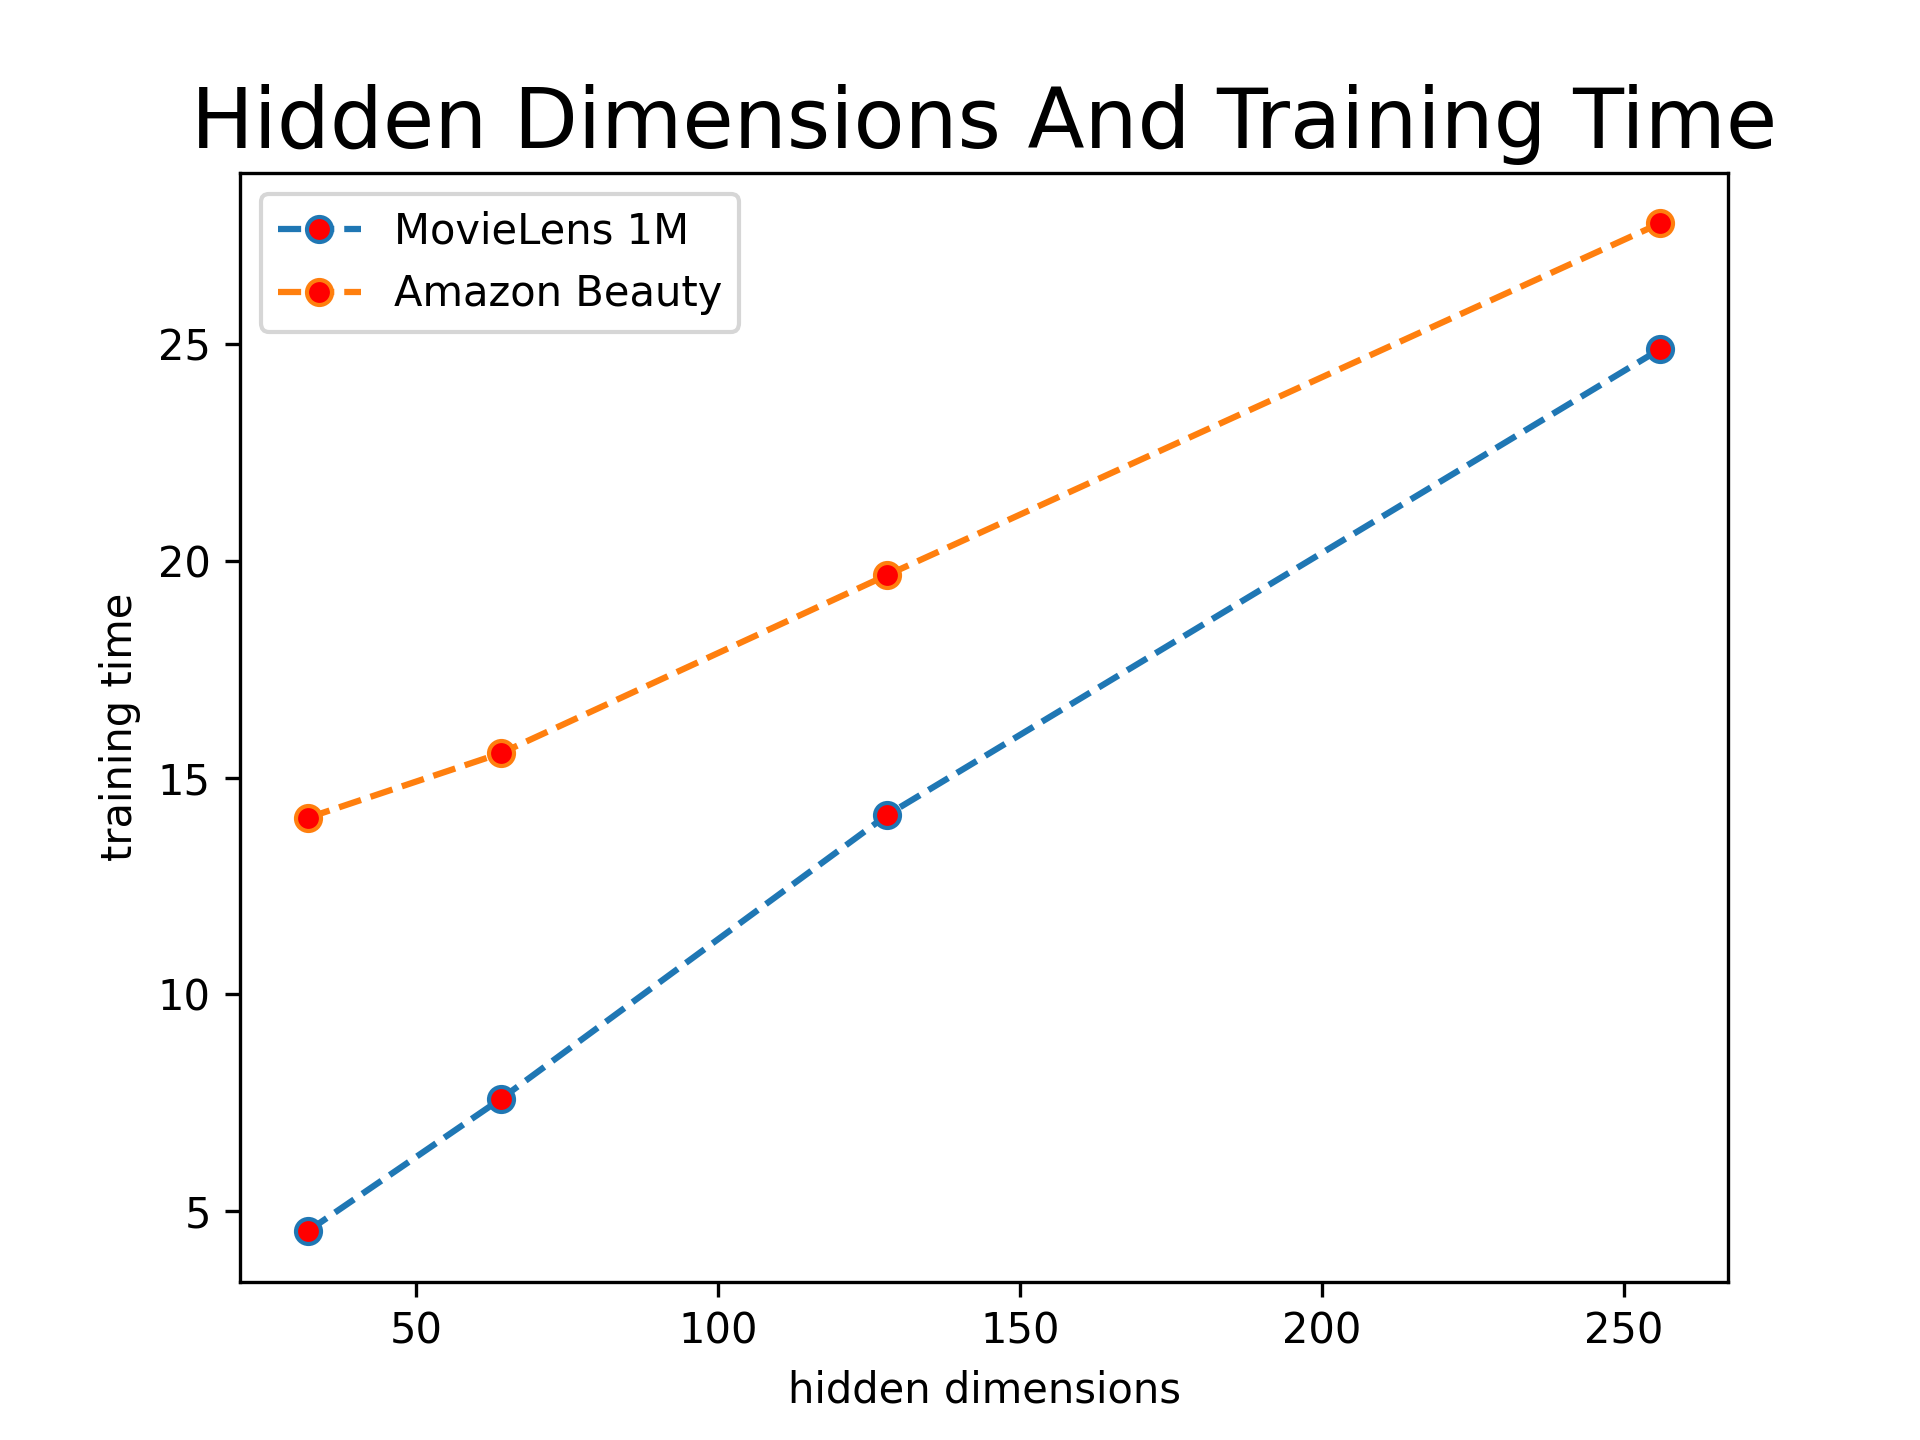
\includegraphics[width=0.8\textwidth]{images/plots/time_hidden_dimensions.png}
\caption{The impact of the hidden dimensions on the training time of our system for both datasets.}
\label{fig:time_hidden_dimensions}
\end{figure}

\begin{table}[htbp!]
\centering
 \begin{tabular}{||c c c c c||} 
 \hline
  & 32 & 64 & 128 & 256 \\ [0.5ex] 
 \hline\hline
 hitrate@10 & 0.748 & 0.7847 & 0.7892 & 0.7875  \\ 
 NDCG@10 & 0.5194 & 0.5698 & 0.5751 & 0.5817   \\
 \hline
 Training Time in hours & 4.54 & 7.59 & 14.14 & 24.88  \\
 \hline
\end{tabular}
\caption{We compare the impact of the dimensions on the training time and performance metrics for the MovieLens 1M dataset.}
\label{tab:performance_dimensions_movielens}
\end{table}

\begin{table}[htbp!]
\centering
 \begin{tabular}{||c c c c c||} 
 \hline
  & 32 & 64 & 128 & 256 \\ [0.5ex] 
 \hline\hline
 hitrate@10 & 0.3956 & 0.4663 & 0.4523 & 0.4381  \\ 
 NDCG@10 & 0.2767 & 0.3034 & 0.3017 & 0.3050     \\
 \hline
 Training Time in hours & 14.07 & 15.56 & 19.67 & 27.78  \\
 \hline
\end{tabular}
\caption{We compare the impact of the dimensions on the training time and performance metrics for the Amazon Beauty dataset.}
\label{tab:performance_dimensions_beauty}
\end{table}

% 1. Say we want to investigate sth. and why it will bring us useful insights.
In our second experiment, we want to investigate how the number of hidden dimensions affects the performance of our hybrid system. We have already discussed in Section~\ref{sec:training_setup} that an increased model size and more training can lead to overfitting and make a model perform worse on new data. However, in the case of BERT, research has shown that we can increase the model size greater than previously thought without hurting performance. The limiting factor is not the size of the model but the hardware limitations and training time~\cite{lan2019albert}. We now want to investigate and discuss the impact of different amounts of hidden dimensions of our hybrid system on the performance and find the optimal number.

% 2. Say how we investigate that thing, i.e., experimental setup.
To experiment, we train our hybrid system with a different number of hidden dimensions. We do so for all of our datasets. Consequently, we use 32, 64, 128, and 256 hidden dimensions. We then observe the time it takes to train the model with the different configurations and measure the performance. 

% 3. Say our results are presented in Material XYZ (plot/table)
We present our results in Figure~\ref{fig:time_hidden_dimensions} and Tables~\ref{tab:performance_dimensions_movielens} and~\ref{tab:performance_dimensions_beauty}.

% 4. describe the results. Just tell us what are the most striking patterns
We can see the measured time it takes to train the system with our two datasets. It takes significantly more time to train the system with the Amazon Beauty dataset. If we look at the training time for the different number of hidden dimensions, we can see that the training time grows less than linear than the number of hidden dimensions. It still takes significantly longer to train the model with more hidden dimensions. We can also see the impact of hidden dimensions on the performance metrics. For the MovieLens 1M dataset, the performance increases as we increase the hidden dimensions and decreases again for 256 hidden dimensions. If we go from 32 to 64 dimensions, the hitrate@10 increases by 4.9\%. However, if we go from 64 to 128 dimensions, the performance only improves by 0.057\%, a small jump. For the Amazon Beauty dataset, we can see a similar effect. Going from 32 to 64 dimensions increases the performance metrics significantly. Increasing the dimensions further only has a small impact on the performance.

% 5. discuss the results. Try to explain what we saw
When we look at both datasets, we can see that the Amazon Beauty dataset is much larger. That explains why it takes more time to train the system with this dataset. We believe that 64 dimensions are the optimal number. More dimensions only have a marginal impact on the performance. On the other hand, reducing the number of dimensions will decrease the performance significantly. This decision however will depend on the requirements of the system. The system administrator has to make a tradeoff between performance and training time. Sometimes it may be warranted to train a system much longer for a very small increase in performance. 